\chapter{Theoretical Framework and Related Work}
\label{ch:framework}

This chapter establishes the conceptual and mathematical foundations required to contextualize this research, transitioning from broad paradigms in Artificial Intelligence to the specific statistical mechanics and adaptive learning strategies underpinning our methodology. We begin by reviewing the fundamental principles of Machine Learning, specifically within the realms of image processing and object classification, before providing a rigorous mathematical treatment of Bayesian Inference, Mixture of Gaussians (MoG) and Gaussian Analysis, including the moment-based and hypothesis-testing tools used throughout this thesis to assess Gaussianity. We then examine the theoretical foundations of covariance estimation in high-dimensional, small-sample regimes---the curse of dimensionality, covariance degeneracy, and the two families of regularisation strategies, spectral conditioning and structured shrinkage, that motivate the specific estimators (diagonal, full, hybrid, shared, OAS, and Ledoit--Wolf) developed in full in Chapter~\ref{methodology}. Finally, we address the challenge of ``catastrophic forgetting" by introducing the Continual Learning (CL) paradigm, describing the datasets utilized and evaluating the state-of-the-art mitigation strategies that provide a performance baseline for the proposed work.

\section{Artificial Intelligence and Machine Learning}

Artificial Intelligence (AI) is a broad field of computer science dedicated to creating systems capable of performing tasks that typically require human intelligence, such as learning, reasoning, perception, and language understanding \cite{RussellNorvig}. Within this domain, Machine Learning (ML) focuses on developing algorithms that allow computers to learn patterns from data without explicit programming. ML systems are generally categorized into three paradigms: Supervised Learning, Unsupervised Learning, and Reinforcement Learning \cite{Bishop2006}.

First, in \textbf{Supervised Learning}, the model learns a mapping from input variables $\mathbf{x}$ to output variables $y$ based on a labeled dataset $\mathcal{D} = \{(\mathbf{x}_i, y_i)\}_{i=1}^N$. The objective is to minimize a loss function that penalizes the discrepancy between the predicted output and the ground truth. This paradigm is typically divided into Classification, where the output is a discrete category, and Regression, where the output is a continuous value.

Second, \textbf{Unsupervised Learning} deals with unlabeled data $\mathcal{D} = \{\mathbf{x}_i\}_{i=1}^N$. Instead of predicting a target, the goal is to discover the underlying structure or distribution of the data. Common tasks include Clustering, which groups similar data points (e.g., K-Means or Gaussian Mixture Models), and Dimensionality Reduction, which projects high-dimensional data into a lower-dimensional space while preserving essential information (e.g., PCA or t-SNE).

Finally, \textbf{Reinforcement Learning} is based on an agent interacting with an environment to maximize a cumulative reward. Unlike supervised learning, the agent is not told which actions to take but must discover them through trial and error. This process is often modeled as a Markov Decision Process (MDP) \cite{Sutton2018}, where the agent transitions between states based on actions, receiving feedback in the form of numerical rewards. The focus is on finding an optimal policy that balances exploration (trying new actions) and exploitation (using known high-reward actions).

\subsection{Deep Learning}

In traditional Machine Learning, the feature extraction step is a manual process where a human expert must identify and define the most relevant characteristics (such as the shape or edges of the car) before passing them to a classification algorithm. In contrast, as shown in figure \ref{fig:deep_learning}, Deep Learning utilizes neural networks to automate this process; the model performs both feature extraction and classification simultaneously, learning to identify complex patterns directly from the input data without human intervention.

Structurally, this shift allows Deep Learning to handle much more complex, high-dimensional data, though it typically requires significantly larger datasets and more computational power to be effective. While traditional Machine Learning depends on the quality of hand-crafted features, Deep Learning architectures—like multi-layered neural networks—are designed to build hierarchical representations of data, progressively moving from low-level pixels to high-level object concepts.

\begin{figure}[ht]
	\centering
	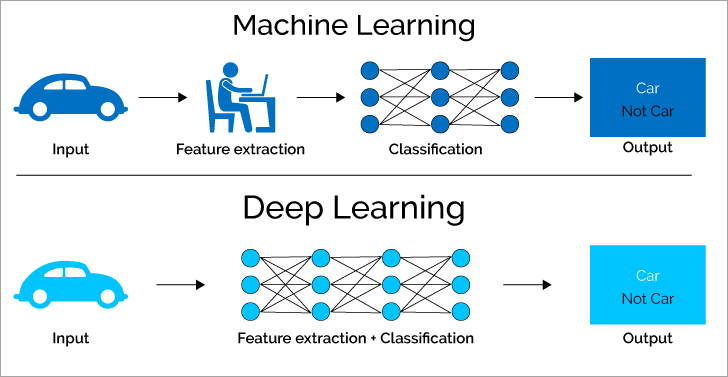
\includegraphics[width=0.7\textwidth]{imagenes/marco/deep.png}
	\caption{Machine Learning and Deep Learning Strategies. Image taken from \cite{deep}.}
	\label{fig:deep_learning}
\end{figure}

\subsection{Computer Vision and Vision Transformers}

Computer Vision is the interdisciplinary subfield of AI that enables computers to gain high-level understanding from digital images or videos, effectively automating tasks performed by the human visual system \cite{Szeliski2010}. While Convolutional Neural Networks (CNNs) \cite{CNN} historically dominated this field, the Transformer architecture---originally developed for Natural Language Processing---has revolutionized visual recognition through the self-attention mechanism \cite{AttentionIsAllYouNeed}.

Vision Transformers (ViT) adapt this architecture by treating an image as a sequence of discrete tokens. As illustrated in Figure \ref{fig:ViTArchitecture}, the process follows a specific pipeline: 

\begin{itemize}
	\item \textbf{Patch Partitioning:} The input image is decomposed into fixed-size patches.
	\item \textbf{Linear Projection:} These patches are flattened and mapped to an embedding space.
	\item \textbf{Positional Encoding:} Since Transformers lack inherent knowledge of spatial structure, learnable position embeddings are added to the patch embeddings.
	\item \textbf{Transformer Encoder:} The resulting sequence is processed through multiple layers of multi-head self-attention and MLP blocks to capture global dependencies.
\end{itemize}

\begin{figure}[ht]
	\centering
	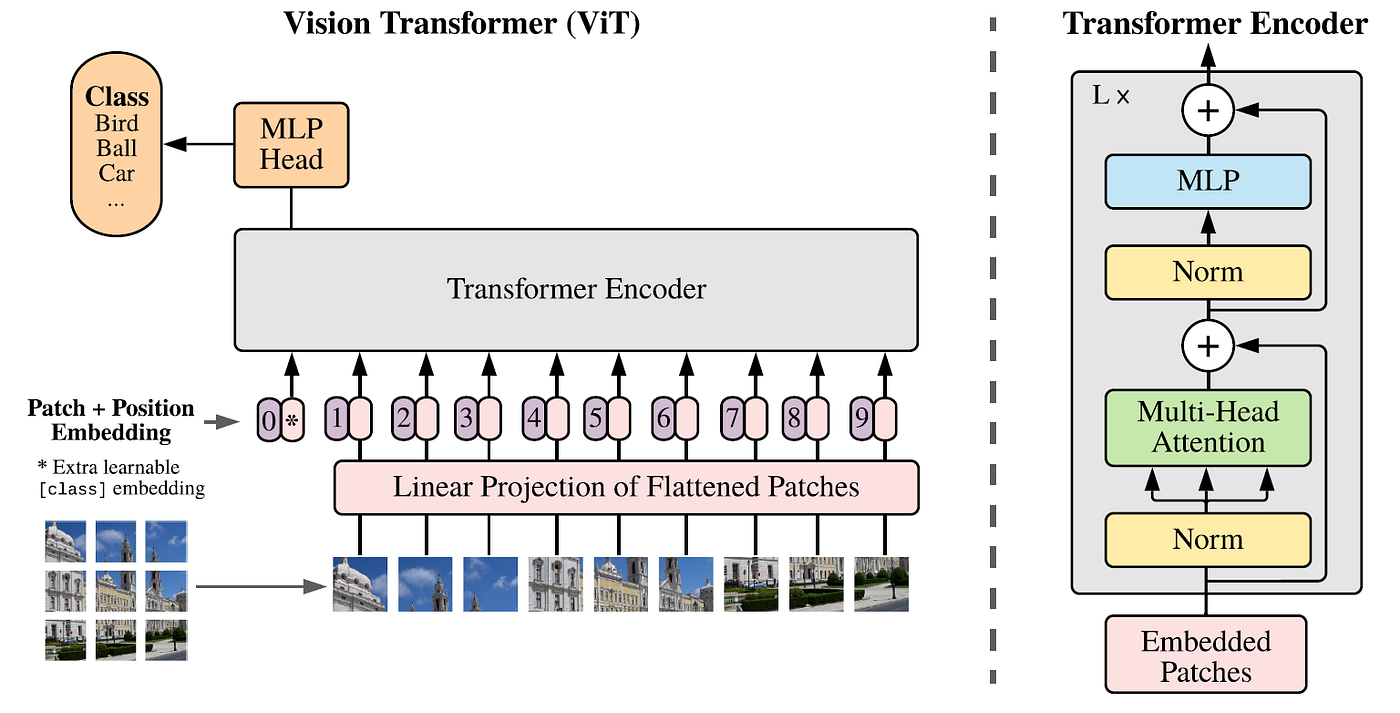
\includegraphics[width=0.7\textwidth]{imagenes/marco/ViT.png}
	\caption{Vision Transformer (ViT) architecture overview. The model processes an image as a sequence of patches through a standard Transformer encoder. Image taken from \cite{AnImageIsWorth}.}
	\label{fig:ViTArchitecture}
\end{figure}

\subsubsection{Object Classification and Representative Power}
The primary objective of the original ViT was \textit{Object Classification}: the fundamental task of assigning a single categorical label to an entire input image. This task serves as the primary benchmark for evaluating the representative power of visual models \cite{Krizhevsky2012}. By processing the global sequence of patches, ViTs have demonstrated an ability to meet or exceed CNN performance, particularly when pre-trained on the large-scale datasets described below.

\subsubsection{Self-Supervised Advancements: DINOv2}

While most datasets rely on explicit human annotations, recent advancements have shifted toward foundational models trained via self-supervised learning (SSL). A prominent representative of this paradigm is \textbf{DINOv2} \cite{oquab2024dinov}, which produces highly robust, multipurpose visual features that exhibit exceptional ``out-of-the-box'' performance across both image-level and pixel-level tasks.

The underlying architecture of DINOv2 relies on a joint \textbf{Student-Teacher self-distillation} framework, building upon DINO \cite{DINO} and iBOT \cite{ibot}. It operates with two parallel networks of identical configuration: a \textit{Student} network $g_{\theta_s}$ and a \textit{Teacher} network $g_{\theta_t}$, whose weights $\theta_t$ are updated as an Exponential Moving Average (EMA) of the student's weights:

\begin{equation}
	\theta_t \leftarrow \lambda \theta_t + (1 - \lambda) \theta_s
\end{equation}

where $\lambda \in [0, 1]$ is a smoothing parameter. During training, the framework optimizes two complementary objectives to learn both global and fine-grained spatial representations:

\begin{itemize}
	\item \textbf{Image-Level Loss (DINO):} The student is fed with both global and local image crops, while the teacher processes only global views. The student is trained to match the teacher's output distribution over a set of virtual prototype vectors, stabilized using an online \textit{Sinkhorn-Knopp centering} algorithm to prevent representation collapse.
	\item \textbf{Patch-Level Loss (iBOT):} To force the model to capture dense, localized features, random patches of the student's global views are masked out. The student must reconstruct the corresponding local patch features produced by the teacher, which receives the fully unmasked global view.
	\item \textbf{KoLeo Regularization:} To ensure that the resulting embeddings are distributed uniformly across the feature space and do not collapse into a narrow cone, DINOv2 incorporates the Kozachenko-Leonenko (KoLeo) differential entropy estimator:
	\begin{equation}
		\mathcal{L}_{\text{KoLeo}} = -\frac{1}{n}\sum_{i=1}^{n} \log \left( \min_{j \neq i} \| \vec{x}_i - \vec{x}_j \|_2 \right)
	\end{equation}
	where $\vec{x}_i$ represents the $\ell_2$-normalized feature vector of the $i$-th image sample in a batch of size $n$.
\end{itemize}	


\subsection{Image Datasets and Benchmarks} 
To rigorously test the robustness and generalization of architectures like ViT, this work utilizes several standardized datasets that vary in scale, stylistic diversity, and granularity.

\subsubsection{The ImageNet Family}
\textbf{ImageNet} \cite{imagenet} is a cornerstone of computer vision, providing over 1.2 million images across 1,000 classes. Its hierarchical structure, based on WordNet, makes it the standard for large-scale classification. To further push the boundaries of model performance, two variants are often employed:
\begin{itemize}
	\item \textbf{ImageNet-21K (and ImageNet-21k-P):} An expansive version containing 14 million images across 21,000 classes \cite{imagenet21k}. The ``P'' version is a cleaned subset designed to make pre-training for models like ViT more accessible.
	\item \textbf{ImageNet-R (Renditions):} A dataset of 30,000 images covering 200 classes in non-photographic styles (e.g., art, sketches). It tests a model's robustness to out-of-distribution data \cite{imagenetR}.
\end{itemize}

\subsubsection{Fine-Grained and Diverse Benchmarks}
Beyond large-scale pre-training, fine-grained classification is evaluated using:

\begin{itemize}
	\item \textbf{CIFAR-100:} Consists of 60,000 low-resolution ($32\times32$) images \cite{cifar100}. It is unique for its two-level hierarchy, where 100 ``fine'' classes are nested within 20 ``coarse'' superclasses, allowing for the evaluation of both specific and broad categorization.
	\item \textbf{Caltech-256:} Provides 30,607 images across 256 categories \cite{caltech256}. It offers greater category diversity and a higher minimum number of images per class than its predecessors, serving as a robust benchmark for generalisation. In this thesis we use the first 250 categories (approximately 28,100 images) so that the resulting class-incremental protocol can be divided into 10 balanced tasks of 25 classes each (see Chapter~\ref{methodology}).
\end{itemize}


\section{Foundations of Probabilistic Modeling}

The convergence of statistical learning theory and high-dimensional data analysis has necessitated the development of robust mathematical frameworks to handle the dual challenges of uncertainty quantification and dimensionality reduction. As modern neural architectures, such as the DINOv2 Vision Transformer, extract increasingly complex representations from datasets like ImageNet-R, the subsequent classification and density estimation layers must be grounded in rigorous probabilistic foundations. 

\subsection{Bayes Classification}

At its core, Bayes classification is rooted in \textbf{Bayes' Theorem}, which provides a mathematical framework for updating the probability of a hypothesis based on observed evidence. For a classification task, we seek the posterior probability $p(y=c \mid \vec{x})$—the probability that an observation belongs to class $c$ given its observed feature vector $\vec{x}$.

Bayes' Theorem is defined as:
\begin{equation}
	p(y=c \mid \vec{x}) = \frac{p(\vec{x} \mid y=c) \, p(y=c)}{p(\vec{x})}
\end{equation}
where:
\begin{itemize}
	\item $p(y=c \mid \vec{x})$ is the \textbf{posterior} probability.
	\item $p(\vec{x} \mid y=c)$ is the \textbf{likelihood} of the data given the class.
	\item $p(y=c)$ is the \textbf{prior} probability of the class.
	\item $p(\vec{x})$ is the \textbf{evidence} or marginal likelihood, acting as a normalization constant.
\end{itemize}

The objective of a Bayes classifier is to minimize the Bayes risk; in the simplest case, this corresponds to assigning the observation to the class that maximizes the posterior probability.

\subsection{Likelihood-Based Classification}

Likelihood inference provides a coherent framework for updating the probability of a hypothesis as more evidence or information becomes available. In contrast to frequentist approaches that treat parameters as fixed but unknown constants, the Bayesian paradigm treats parameters as random variables characterized by probability distributions.

The connection between Bayes' Theorem and likelihood-based classification lies in the \textbf{Maximum A Posteriori (MAP)} decision rule. Since the evidence $p(\vec{x})$ is constant across all classes for a given observation, the classification decision depends solely on the product of the likelihood and the prior:
\begin{equation}
	p(y=c \mid \vec{x}) \propto p(\vec{x} \mid y=c) \, p(y=c).
\end{equation}

A generative modeling framework can be adopted and class-conditional Gaussian feature distributions can be assumed:
\begin{equation}
	p(\vec{x} \mid y=c)
	=
	\mathcal{N}(\vec{x} \mid \boldsymbol{\mu}_c, \boldsymbol{\Sigma}_c),
\end{equation}
where $\vec{x} \in \mathbb{R}^d$ represents the feature vector, $\boldsymbol{\mu}_c$ is the class mean vector, and $\boldsymbol{\Sigma}_c \succ 0$ is the covariance matrix.

Classification can be performed via MAP inference by maximizing the log-posterior:
\begin{equation}
	\hat{y}
	=
	\arg\max_{c \in \mathcal{Y}}
	\left[
	\log p(\vec{x} \mid y=c) + \log \pi_c
	\right],
\end{equation}
where $\pi_c = p(y=c)$ denotes the class prior.

Substituting the multivariate Gaussian density into the MAP rule, the decision rule becomes equivalent to:
\begin{equation}
	\hat{y}
	=
	\arg\min_{c}
	\left[
	(\vec{x}-\boldsymbol{\mu}_c)^T
	\boldsymbol{\Sigma}_c^{-1}
	(\vec{x}-\boldsymbol{\mu}_c)
	+
	\log |\boldsymbol{\Sigma}_c|
	-
	2\log \pi_c
	\right].
\end{equation}

\subsubsection{Mixture of Gaussians (MoG)} 

A Mixture of Gaussians models a complex probability density as a convex combination of $K$ distinct Gaussian components. This approach is fundamental for clustering and density estimation in multi-modal distributions. Therefore, to capture multimodal feature distributions, the class-conditional model can be extended to a mixture:

\begin{equation}
	p(\vec{x} \mid y=c)
	=
	\sum_{k=1}^{K_c}
	\alpha_{c,k}
	\mathcal{N}(\vec{x} \mid \boldsymbol{\mu}_{c,k}, \boldsymbol{\Sigma}_{c,k}),
\end{equation}
where $\alpha_{c,k} \ge 0$ and $\sum_k \alpha_{c,k} = 1$.

The MAP decision rule becomes
\begin{equation}
	\hat{y}
	=
	\arg\max_c
	\left[
	\log
	\left(
	\sum_{k=1}^{K_c}
	\alpha_{c,k}
	\mathcal{N}(\vec{x} \mid \boldsymbol{\mu}_{c,k}, \boldsymbol{\Sigma}_{c,k})
	\right)
	+
	\log \pi_c
	\right].
\end{equation}

\subsection{Gaussianity Assumptions and Analysis}
In the context of generative modeling for foundation feature spaces, the validity of the Bayes classifier depends on how well the class-conditional Gaussian distributions approximate the true data distribution. The following analytical framework establishes the statistical basis for these assumptions.

\subsubsection{Principal Component Analysis}
\label{sec:marco:pca}

Principal Component Analysis (PCA) is a linear dimensionality-reduction technique that finds an orthonormal basis for the data by diagonalising the empirical covariance matrix~\cite{jolliffe2002principal}. Given a centred data matrix $\mathbf{X} \in \mathbb{R}^{N \times d}$ (zero-mean columns), the empirical covariance is

\begin{equation}
\mathbf{S} = \frac{1}{N-1}\mathbf{X}^{T}\mathbf{X}.
\end{equation}

Its eigendecomposition $\mathbf{S} = \mathbf{P}\boldsymbol{\Lambda}\mathbf{P}^{T}$ yields orthonormal eigenvectors $\mathbf{P} = [\mathbf{p}_1, \ldots, \mathbf{p}_d]$ sorted so that the corresponding eigenvalues satisfy $\lambda_1 \ge \lambda_2 \ge \cdots \ge \lambda_d \ge 0$. Each eigenvector $\mathbf{p}_i$ is a \emph{principal component} (PC), and $\lambda_i$ equals the variance of the data projected onto $\mathbf{p}_i$.

\paragraph{Dimensionality reduction.}
Retaining only the leading $k$ eigenvectors defines the projection matrix $\mathbf{P}_k = [\mathbf{p}_1, \ldots, \mathbf{p}_k] \in \mathbb{R}^{d \times k}$. A new observation $\vec{x} \in \mathbb{R}^d$ is mapped to a $k$-dimensional representation via

\begin{equation}
\tilde{\vec{x}} = \mathbf{P}_k^{T}(\vec{x} - \boldsymbol{\mu}),
\label{eq:pca_project}
\end{equation}

where $\boldsymbol{\mu}$ is the global mean estimated from the training corpus. The resulting coordinates $\tilde{\vec{x}}$ are decorrelated: $\operatorname{Cov}(\tilde{\vec{x}}) = \operatorname{diag}(\lambda_1, \ldots, \lambda_k)$. The fraction of total variance preserved by the projection is

\begin{equation}
R(k) = \frac{\sum_{i=1}^{k}\lambda_i}{\sum_{i=1}^{d}\lambda_i}.
\end{equation}

\paragraph{Optimality and geometric interpretation.}
Among all rank-$k$ linear projections, PCA minimises the mean-squared reconstruction error and maximises the variance of the projected data (Eckart--Young theorem~\cite{eckart1936approximation}). Geometrically, the projected subspace aligns with the axes of the data ellipsoid along which the observations spread most.

\paragraph{Application to high-dimensional embeddings.}
When the original dimension $d$ is large (e.g.\ $d=768$ for DINOv2 ViT-B/14) but the data occupy a low-dimensional subspace---as evidenced by rapid eigenvalue decay---reducing to $k \ll d$ dimensions before downstream classification offers two complementary benefits: (i) it concentrates the discriminative signal in fewer coordinates, potentially improving the accuracy of subsequent covariance estimators; and (ii) it reduces computational cost by a factor of $\mathcal{O}((d/k)^2)$ for quadratic (Mahalanobis) classifiers. The trade-off is that components beyond $k$ are discarded, which may remove residual discriminative information if the spectrum does not decay quickly enough.

\subsubsection{Spectral Decay and Effective Dimensionality}

The practical validity of high-dimensional Gaussian modeling is further supported by examining the spectral structure of the feature space through Principal Component Analysis (PCA). The covariance of the class-mean-centred embeddings can be decomposed as $\boldsymbol{\Sigma} = \mathbf{P}\boldsymbol{\Lambda}\mathbf{P}^T$, where the diagonal of $\boldsymbol{\Lambda}$ contains the eigenvalues $\lambda_1 \ge \lambda_2 \ge \dots \ge \lambda_d \ge 0$ and $\mathbf{P}$ holds the corresponding orthonormal eigenvectors.

\paragraph{Variance concentration.}
If the eigenvalue spectrum decays steeply---most variance is explained by the first $k \ll d$ components---then the effective dimensionality of the feature distribution is much lower than the nominal $d$. Concretely, the fraction of variance explained by the leading $k$ components is $\sum_{i=1}^{k}\lambda_i \,/\, \sum_{i=1}^{d}\lambda_i$.


\subsubsection{Univariate Gaussianity}

A second layer of theoretical justification involves examining the univariate properties of individual feature components.

\paragraph{Kurtosis} This statistic measures the ``tailedness'' and peakedness of a probability distribution relative to a normal distribution \cite{joyce2011kurtosis}. As illustrated in Figure \ref{fig:kurtosis}, a perfectly Gaussian distribution has an excess kurtosis of zero (mesokurtic). Distributions with high kurtosis (leptokurtic, $Kurtosis > 0$) exhibit sharper peaks and heavier tails, indicating a higher concentration of data around the mean and a greater likelihood of extreme outliers. Conversely, low kurtosis (platykurtic, $Kurtosis < 0$) indicates a flatter peak and thinner tails. Empirical evidence suggests that for many foundation model embeddings, kurtosis values typically fall within the range of $[-1, 1]$, justifying the Gaussian approximation.


\begin{figure}[ht]
	\centering
	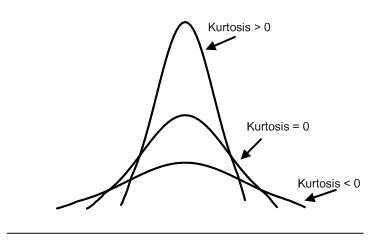
\includegraphics[width=0.37\textwidth]{imagenes/marco/kurtosis.png}
	\caption{Visual representation of kurtosis levels: leptokurtic ($>0$), mesokurtic ($=0$) and platykurtic ($<0$) distributions \cite{joyce2011kurtosis}.}
	\label{fig:kurtosis}
\end{figure}

\paragraph{Skewness} This measure quantifies the asymmetry of a distribution around its mean. As shown in Figure \ref{fig:skewness}, a symmetric distribution (center) is a fundamental assumption of the Gaussian model, implying that the mean $\boldsymbol{\mu}_c$, median, and mode coincide, providing an adequate representation of the class prototype within the embedding space. A positive skew (right) indicates a distribution with a long tail extending toward higher values, while a negative skew (left) indicates a long tail extending toward lower values. Significant skewness would suggest that the class-conditional mean is no longer a central representation of the feature distribution.

\begin{figure}[ht]
	\centering
	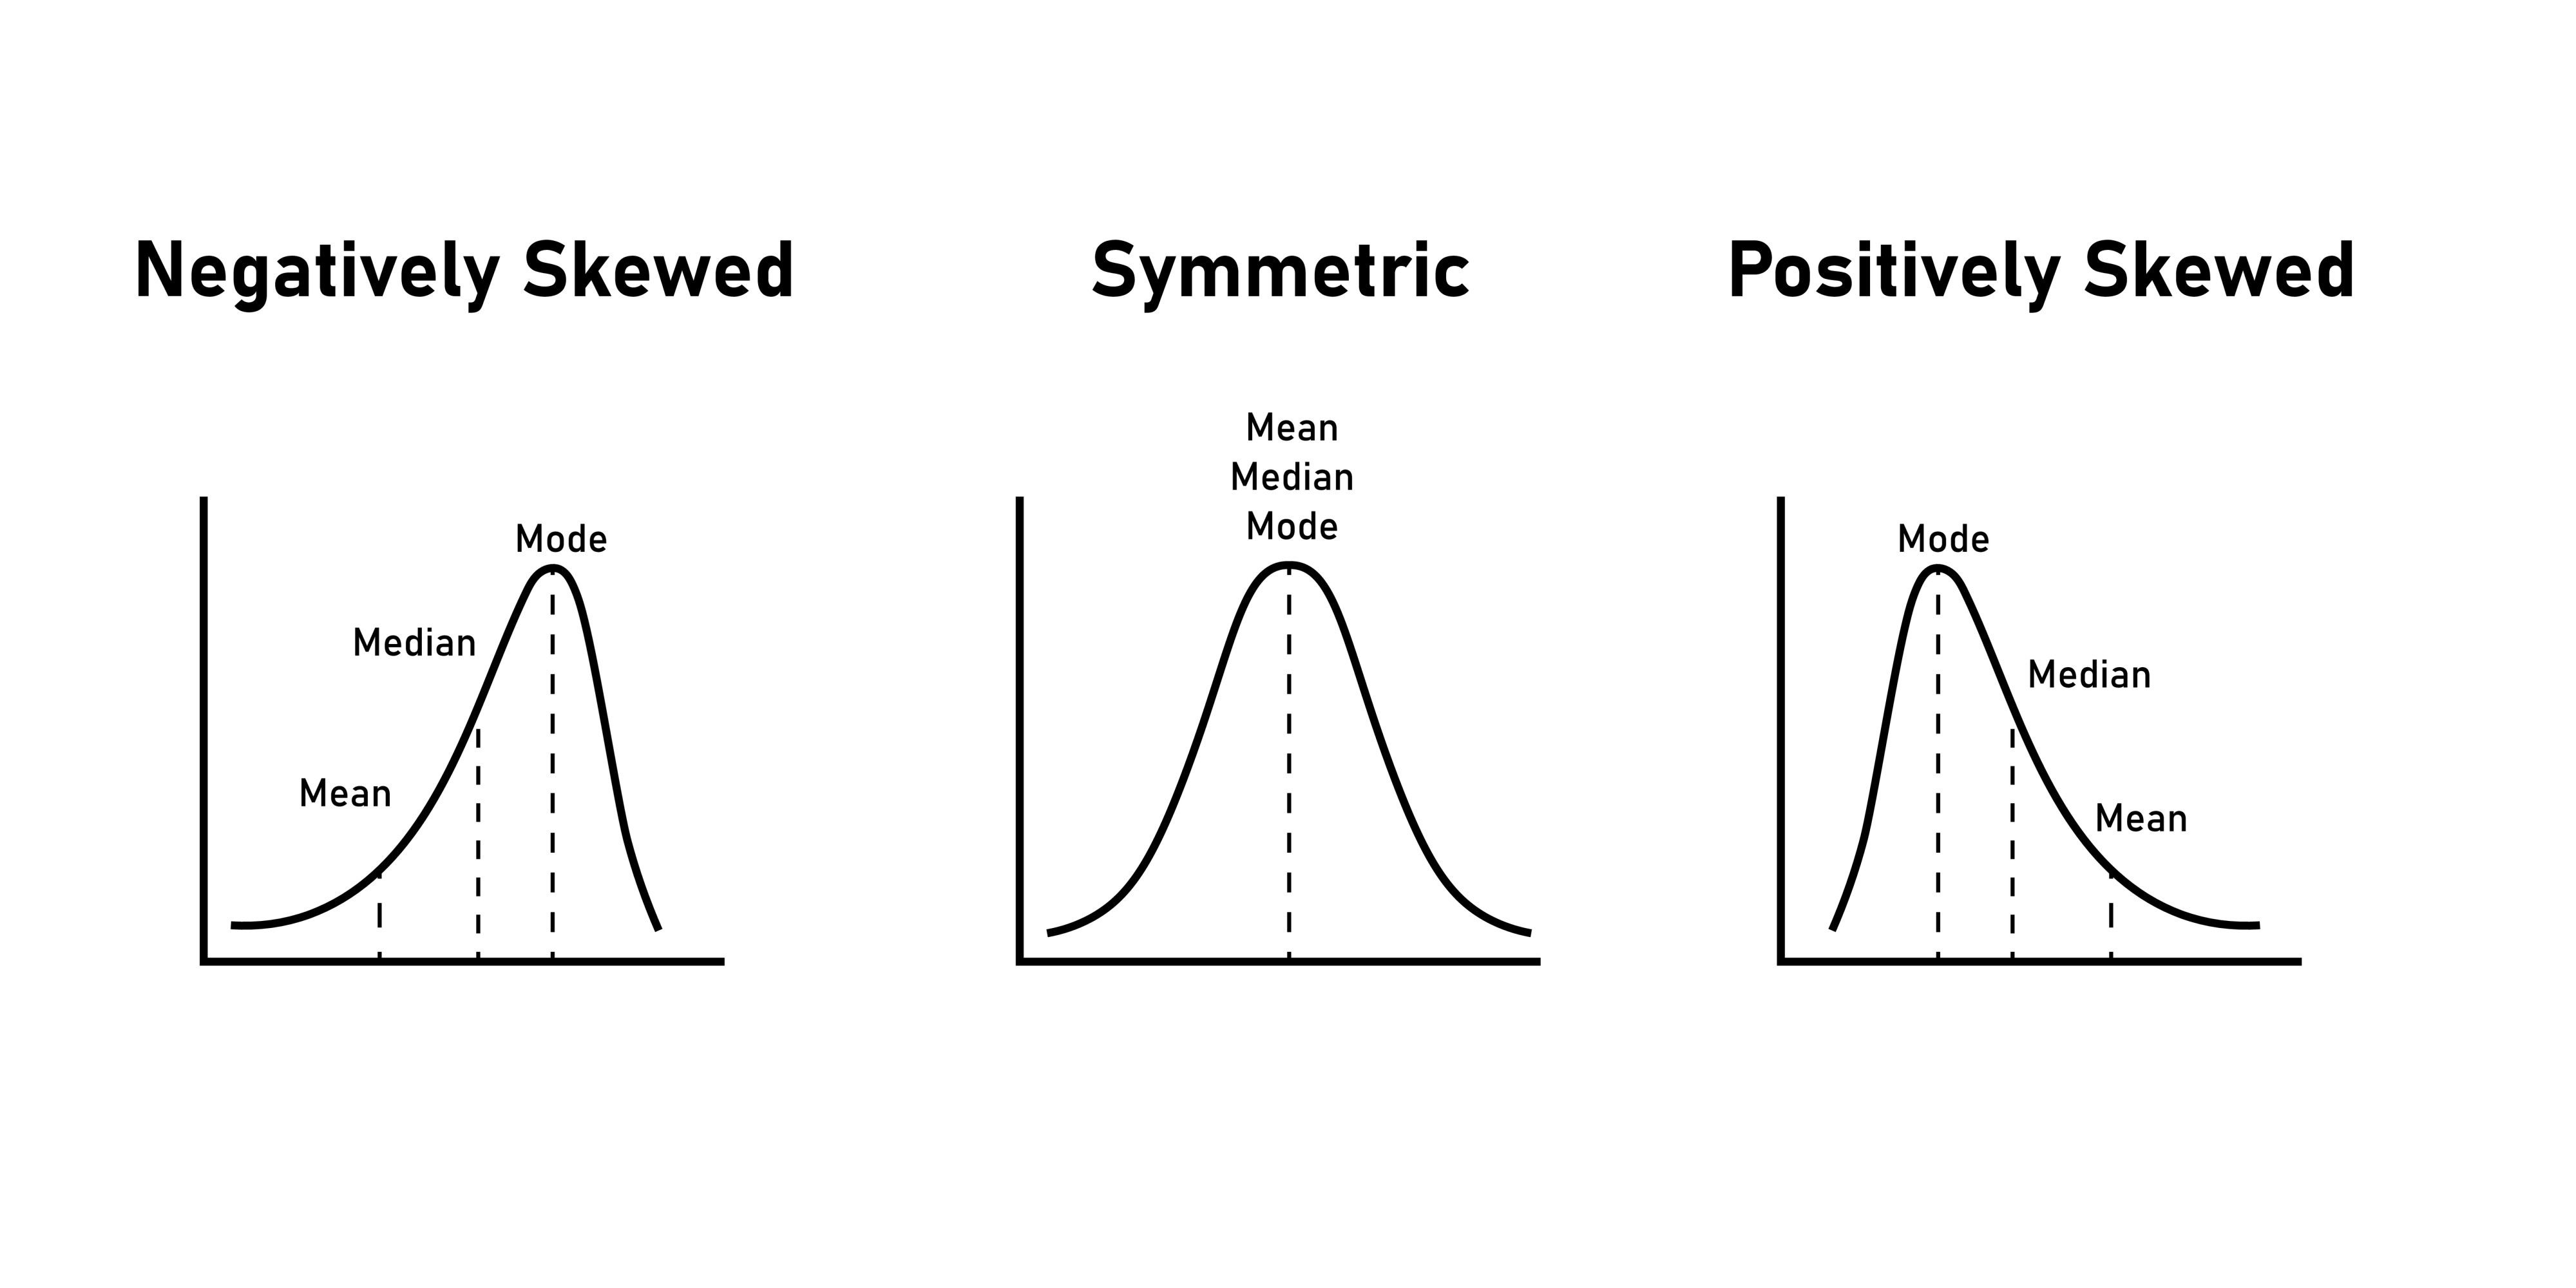
\includegraphics[width=0.7\textwidth]{imagenes/marco/skeweness.jpg}
	\caption{Comparison of negatively-skewed, symmetric and positively-skewed distributions \cite{pearson1895skewness}.}
	\label{fig:skewness}
\end{figure}


\subsubsection{Multivariate Gaussianity}
\label{sec:method:gaussianity:hz_theory}

Per-dimension normality is necessary but not sufficient for the joint $d$-dimensional distribution to be Gaussian. The Henze--Zirkler (HZ) test~\cite{henze1990class} is an omnibus multivariate diagnostic that addresses this gap by comparing the empirical characteristic function of the data against the theoretical characteristic function of a multivariate normal distribution.

Given $n$ centred samples $\vec{z}_i = \vec{x}_i - \hat{\boldsymbol{\mu}}_c$ and a smoothing bandwidth $b > 0$, the test statistic is built from three terms evaluated using the squared Mahalanobis distances $d_M^2(\cdot,\cdot)$ induced by the class covariance $\boldsymbol{\Sigma}_c$:

\begin{equation}
	A = \frac{1}{n^2} \sum_{j=1}^{n} \sum_{k=1}^{n} e^{-\frac{b^2}{2}d_M^2(\vec{z}_j, \vec{z}_k)},
\end{equation}
\begin{equation}
	B = \frac{2}{n}(1+b^2)^{-d/2} \sum_{j=1}^{n} e^{-\frac{b^2}{2(1+b^2)}d_M^2(\vec{z}_j, \vec{0})},
\end{equation}
\begin{equation}
	C = (1+2b^2)^{-d/2}.
\end{equation}

Term $A$ measures the average pairwise kernel similarity of the observed samples; term $B$ quantifies how consistently the empirical density decays away from the class centroid compared to a Gaussian; and term $C$ is the asymptotic self-similarity constant of a true $d$-dimensional Gaussian. The final statistic is:
\begin{equation}
	T_{n,b} = n \cdot \left[ A - B + C \right].
\end{equation}

Under the null hypothesis of multivariate normality, $T_{n,b}$ converges to a fixed value close to $1$; departures above $1$ indicate that the data is more structured (tighter clusters or heavier tails) than a Gaussian. The bandwidth $b$ controls the resolution of the characteristic function comparison and is set optimally as a function of $n$ and $d$.

\subsection{Covariance Estimation in High-Dimensional Spaces}

A fundamental challenge in multivariate statistical analysis and pattern recognition is the estimation of the covariance matrix $\boldsymbol{\Sigma} \in \mathbb{R}^{d \times d}$ from a finite set of $n$ observations. In classical low-dimensional regimes, where the sample size $n$ is much larger than the feature dimension $d$ ($n \gg d$), the empirical Sample Covariance Matrix (SCM) acts as a reliable, unbiased estimator. However, modern engineering applications—such as analyzing high-dimensional deep feature representations—frequently operate in the ``high-dimension, small-sample-size'' (HDSS) regime, where $d$ is of the order of hundreds or thousands, while $n$ remains strictly limited.

Under these conditions, classical multivariate analysis suffers severely from the \textit{curse of dimensionality}, leading to critical theoretical and numerical breakdowns in statistical modeling.

\subsubsection{The Curse of Dimensionality and Covariance Degeneracy}

When the dimensionality $d$ scales while the sample size $n$ remains fixed or grows at a slower rate, several geometric and algebraic anomalies emerge:

\begin{itemize}
	\item \textbf{Singularity and Rank Deficiency:} Structurally, the SCM is calculated as the sum of $n$ outer products of centered data vectors. Consequently, the maximum rank of the SCM is bounded by $\min(n-1, d)$. In the typical HDSS scenario where $n < d$, the SCM has at least $d - n + 1$ zero eigenvalues. The resulting matrix is singular (rank-deficient) and cannot be inverted.
	
	\item \textbf{Loss of Negative Log-Likelihood and Distance Metrics:} Many fundamental statistical classifiers and density estimators—such as Gaussian Discriminant Analysis (GDA) or Mahalanobis distance formulations—depend heavily on the precision matrix (the inverse covariance, $\boldsymbol{\Sigma}^{-1}$) and the log-determinant $\ln|\boldsymbol{\Sigma}|$. When the estimated covariance is singular, the log-determinant diverges to $-\infty$, and the precision matrix is undefined, rendering density estimation mathematically impossible.
	
	\item \textbf{Eigenvalue Distortion (Spreading Phenomenon):} Even in moderately high dimensions where $n \ge d$ and the SCM is technically invertible, the sample eigenvalues do not converge to their true counterparts. As proved in random matrix theory (e.g., the Marčenko-Pastur law \cite{MarPas67}), high-dimensional sample eigenvalues exhibit severe bias: the largest eigenvalues are systematically overestimated, while the smallest eigenvalues are underestimated. This artificial dispersion distorts the perceived geometric structure of the data.
\end{itemize}

\subsubsection{Theoretical Foundations of Regularization}

To overcome the numerical and structural instability of the empirical SCM in high dimensions, the theoretical framework must transition from pure maximum likelihood estimation toward \textit{regularization}. The conceptual objective is to trade a manageable amount of bias for a drastic reduction in estimator variance.

Conceptually, these regularized estimation strategies fall into two primary paradigms:

\begin{enumerate}
	\item \textbf{Spectral Regularization and Conditioning:} These approaches directly manipulate the empirical eigenspectrum. By placing a lower bound on near-zero eigenvalues or adding a perturbation matrix (e.g., diagonal loading), they artificially bound the condition number of the matrix. This guarantees strict positive definiteness ($\boldsymbol{\Sigma} \succ 0$), ensuring that the precision matrix remains numerically stable during inversion.
	
	\item \textbf{Structured Shrinkage:} Shrinkage theory, pioneered by Stein's loss formulations, constructs an estimator as a convex combination of the high-variance SCM and a low-variance structured ``target'' matrix (such as the identity matrix or a diagonal variance matrix). By shrinking the empirical estimator toward a well-behaved target, these methods systematically pull the distorted, spread-out eigenvalues back toward their true mean, minimizing the expected mean squared error.
\end{enumerate}


\section{Continual Learning}

Continual Learning (CL), also known as lifelong learning, constitutes the core focus of this work. It represents a machine learning paradigm designed to handle the progressive acquisition of knowledge from sequences of tasks or data streams over time. As illustrated in Figure \ref{fig:task_time}, a \textbf{task} in this context is defined as a specific learning experience or dataset –such as Task A, B, or C. Each task is potentially characterized by unique data distributions or objectives, as symbolized by the varying shapes (e.g., circles vs. hearts) above the task labels. 

Unlike conventional training approaches that rely on a fixed dataset and a stationary environment, CL emphasizes the arrival of these tasks at distinct intervals along the \textbf{time} axis. This sequential arrival requires the model to be inherently non-stationary, adapting its internal representations as environments evolve. The primary challenge in this paradigm lies in the ongoing integration of new information from a current task (e.g., Task B) while simultaneously preserving the knowledge previously acquired from Task A.

\begin{figure}[ht]
	\centering
	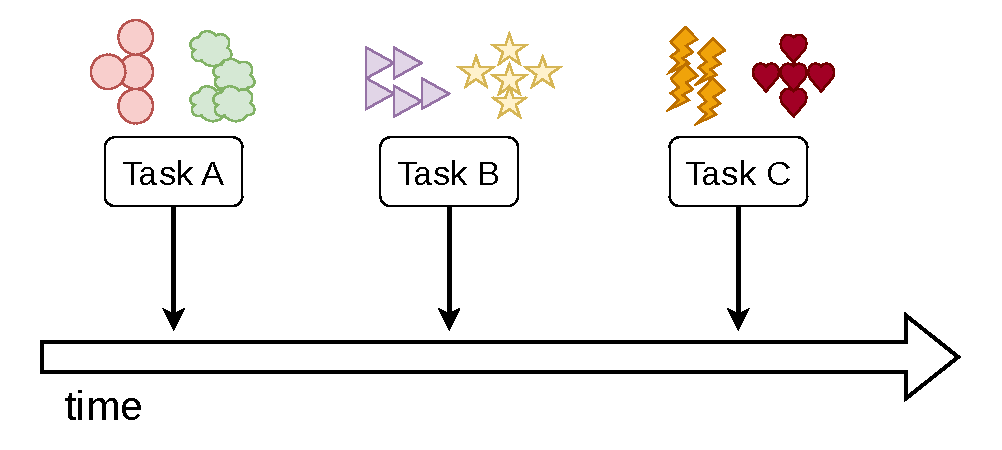
\includegraphics[width=0.75\textwidth]{imagenes/marco/Adaptation.pdf}
	\caption{A sequential task arrival model for Continual Learning, depicting the transition from Task A to Task C over time, where each task represents a unique set of features or data distributions.}
	\label{fig:task_time}
\end{figure}

Without specific architectural or algorithmic safeguards, this sequential learning process inevitably triggers \textbf{catastrophic forgetting} \cite{CL}. This phenomenon occurs when the assimilation of new knowledge leads to the degradation or total loss of prior learning. As illustrated in Figure \ref{fig:catastrophic_forgetting}, the dilemma of forgetting becomes apparent when a \textit{New Object Class} is introduced to an existing classifier, forcing a choice between two traditional but flawed strategies:

\begin{itemize}
	\item \textbf{Fine-Tuning:} Updating the model using only the current task data is computationally efficient but leads directly to catastrophic forgetting \cite{CL}. Because the optimization process focuses solely on the new objective, the internal representations associated with previously learned classes are overwritten, causing the model to lose its original predictive capabilities.
	
	\item \textbf{Retraining from Scratch:} While joint training on the full historical dataset ($\mathcal{D}_{old} \cup \mathcal{D}_{new}$) technically prevents forgetting, it faces two significant hurdles. First is the issue of \textbf{Data Privacy and Availability}: in many real-world scenarios, the original data $\mathcal{D}_{old}$ is often deleted or inaccessible due to privacy regulations. Second is the \textbf{Computational Bottleneck}: as the system's lifespan increases, the cumulative dataset grows, making the energy and time required to retrain the model unsustainable in continuously evolving environments.
\end{itemize}

\begin{figure}[ht]
	\centering
	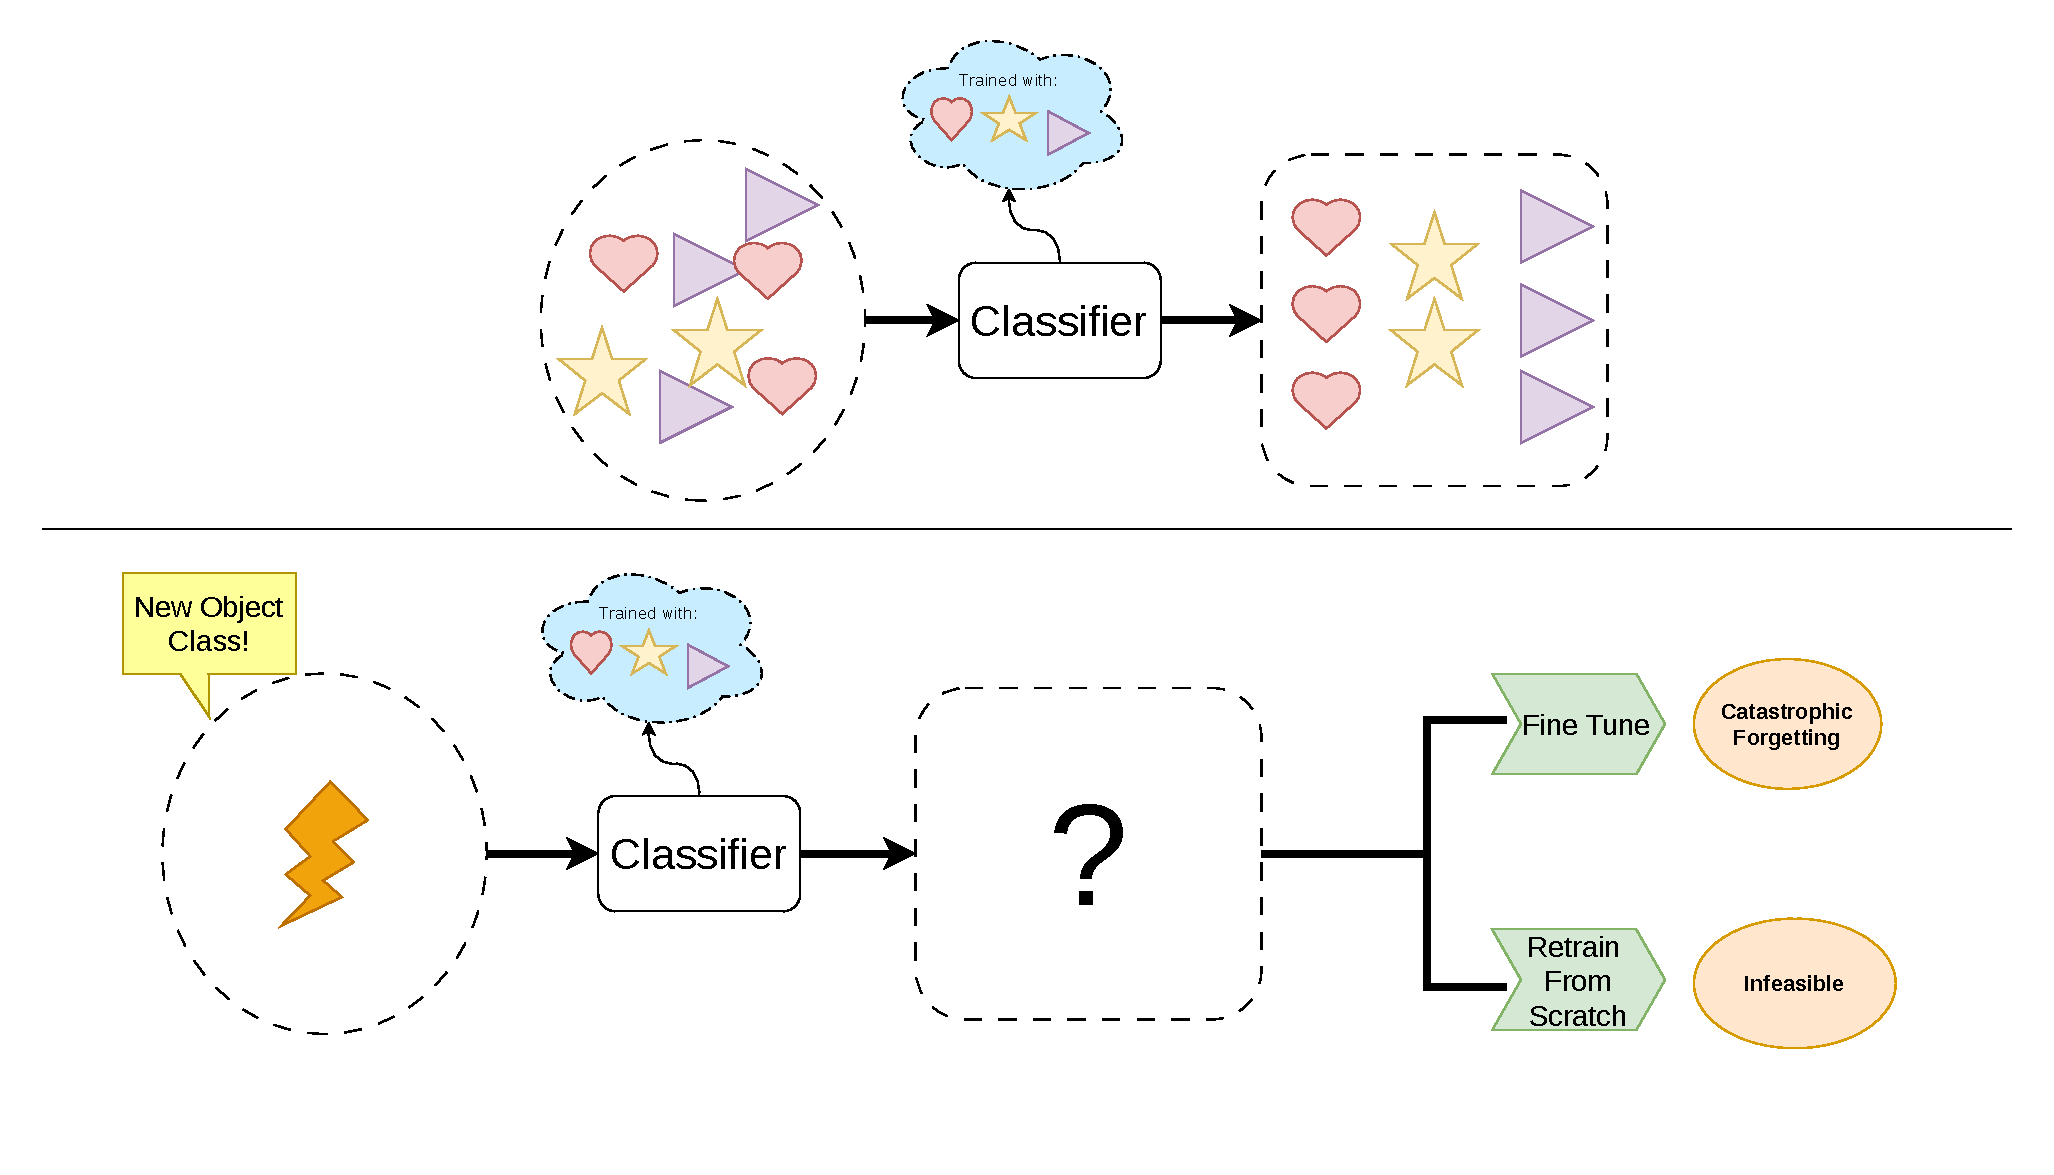
\includegraphics[width=0.8\textwidth]{imagenes/marco/Catastrophic_forgetting.pdf}
	\caption{Standard Object Classifier comparison. The upper path shows standard inference, while the lower path illustrates the dilemma when a new class is introduced: the trade-off between catastrophic forgetting via fine-tuning and the infeasibility of retraining from scratch.}
	\label{fig:catastrophic_forgetting}
\end{figure}

\subsection{Elasticity and Plasticity} 
A central concept in continual learning is the balance between elasticity and plasticity. \textbf{Plasticity} refers to the ability of a model to adapt rapidly to new information, ensuring that it can effectively learn novel tasks. \textbf{Elasticity} (or stability), in contrast, emphasizes preserving the parameters and representations that are crucial for retaining old knowledge \cite{API}. Achieving an appropriate equilibrium between these two properties is known as the \textbf{stability–plasticity dilemma} \cite{CL}.

\subsection{Main Paradigms} 
As shown in Figure \ref{fig:task_vs_class}, two principal paradigms define how continual learning problems are formulated. \textbf{Task-incremental learning (Task-IL)} assumes that the task identity is available during inference, allowing for task-specific components to be isolated \cite{task_il}. \textbf{Class-incremental learning (Class-IL)}, on the other hand, does not provide the task identity at test time, requiring the model to distinguish between all classes seen across all tasks simultaneously \cite{masana_class_il}.

\begin{figure}[ht]
	\centering
	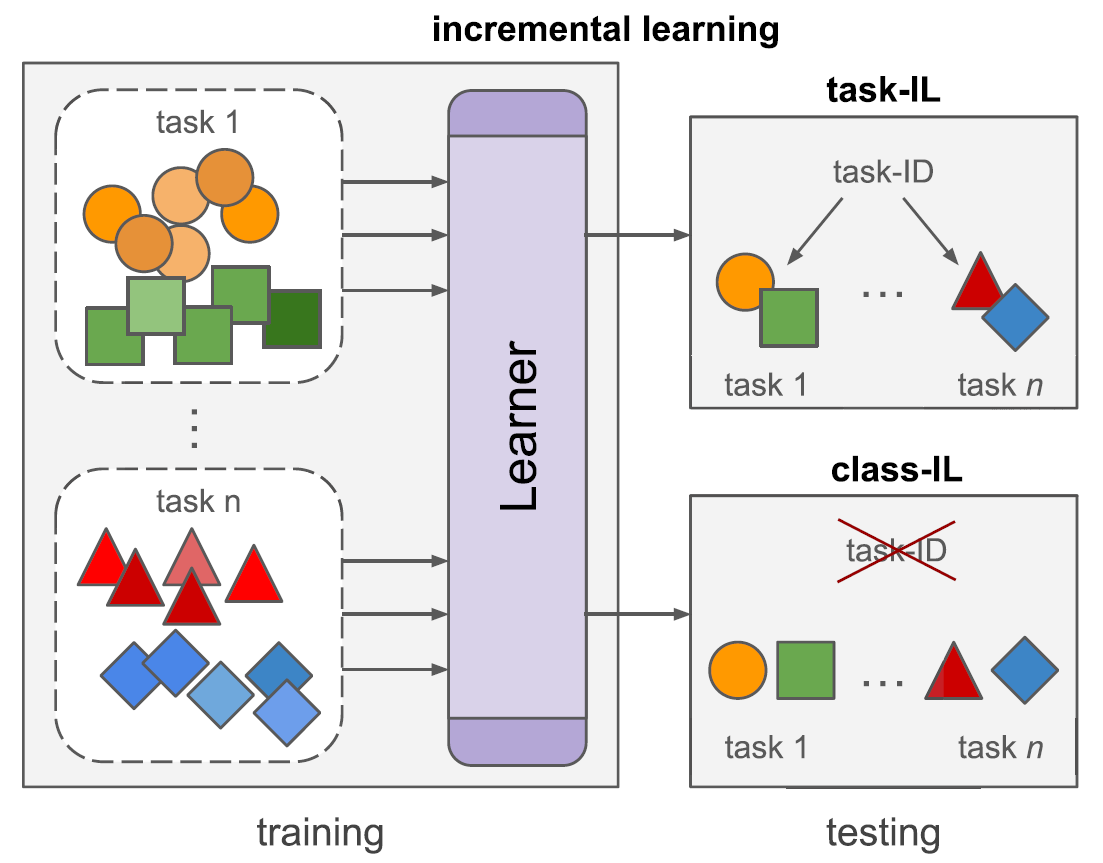
\includegraphics[width=0.5\textwidth]{imagenes/marco/CI_learning_survey_fig1.png}
	\caption{Class and Task Incremental Learning. Image taken from \cite{masana_class_il}.}
	\label{fig:task_vs_class}
\end{figure}

\subsection{Mitigation Strategies}
To address the stability-plasticity dilemma, we categorize existing CL strategies into four main families: rehearsal-based, regularization-based, architecture-based, and representation-based (specifically prompt-based) methods. Additionally, emerging paradigms focus on classifier adaptation over frozen backbones.

\subsubsection{Rehearsal Methods}
To preserve past performance, these methods reuse samples from previously learned tasks while training on the current task.
\begin{itemize}
	\item \textbf{Experience Replay (ER)} \cite{Chaudhry2019ContinualLW}: Maintains a small episodic memory buffer containing a sample of old, representative examples to be interleaved with new data.
	\item \textbf{Average Gradient Episodic Memory (A-GEM)} \cite{agem}: Improves efficiency by using the buffer to constrain the direction of parameter updates, ensuring they do not interfere with past tasks.
	\item \textbf{Dark Experience Replay (DER)} \cite{buzzega2020darkexperiencegeneralcontinual}: Enhances ER by incorporating knowledge distillation on the logits of replayed examples to preserve the ``dark knowledge'' of the model.
	\item \textbf{Generative Replay} \cite{generative_features}: A non-data-storing method where a generator is trained to produce synthetic features or samples of previously learned classes, avoiding the privacy concerns of raw data storage.
\end{itemize}

\subsubsection{Regularization Methods}
These methods limit updates to parameters identified as important for prior learning by introducing penalty terms in the loss function.
\begin{itemize}
	\item \textbf{Elastic Weight Consolidation (EWC)} \cite{Kirkpatrick_2017}: Identifies critical parameters using the Fisher Information Matrix and restricts their movement during new task training.
	\item \textbf{Synaptic Intelligence (SI)} \cite{zenke2017continuallearningsynapticintelligence}: Calculates importance weights online by accumulating their contribution to the reduction of the loss.
	\item \textbf{Learning Without Forgetting (LwF)} \cite{li2017learningforgetting}: A functional regularization method that uses knowledge distillation to ensure the model's outputs for new data remain consistent with the previous model's predictions.
	\item \textbf{Adaptive Plasticity Improvement (API)} \cite{API}: Enforces an update direction orthogonal to the important subspaces of previous tasks using Dual Gradient Projection Memory (Dual-GPM).
\end{itemize}

\subsubsection{Architecture-based Methods}
These methods mitigate forgetting by modifying the network architecture to increase or reorganize its capacity.
\begin{itemize}
	\item \textbf{Parameter Isolation} \cite{10.5555/3454287.3455512}: Identifies and freezes parameters important for previous tasks---often through pruning or gradient masking---so only a subset of weights is updated for the current task.
	\item \textbf{Dynamic Expansion}: Expands the model architecture as new tasks arrive. For instance, DER~\cite{Yan2021DERDE} uses an expandable super-feature extractor followed by pruning, while DEN~\cite{Yoon2017LifelongLW} expands the network dynamically only when the current capacity is insufficient.
\end{itemize}

\subsubsection{Representation and Prompt-based Methods}
The emergence of foundation models (e.g., ViTs) has enabled parameter-efficient fine-tuning (PEFT) where the backbone remains frozen and learning is contained within small, task-specific parameters (``prompts'').
\begin{itemize}
	\item \textbf{Learning to Prompt (L2P)} \cite{wang2022learning}: Uses a query-based prompt pool where prompts are selected based on the similarity between input embeddings and learned keys.
	\item \textbf{Dual Prompt} \cite{wang2022dualprompt}: Refines L2P by separating prompt-based representations into complementary components: fixed G-prompts (General) and task-specific E-prompts (Expert).
	\item \textbf{CODA-Prompt} \cite{Smith_2023_CVPR}: Introduces a fully differentiable scheme where the prompt is a weighted sum of components dynamically calculated via attention mechanisms.
	\item \textbf{Advanced Prompting}: Recent extensions adapt prompt engineering to parameter-efficient and distributed settings. Specifically, \textbf{InFLoRA} \cite{liang2024inflora} and \textbf{DOLFIN} \cite{dolfin} apply low-rank adaptation and distributed learning, while \textbf{APT} \cite{Chen_2025_ICCV} injects key-value tokens directly into transformer layers to minimize inference overhead.
\end{itemize}

\subsubsection{Classifier Adaptation on Frozen Representations}
A complementary line of work investigates classifier adaptation on top of frozen feature extractors, remaining fundamentally discriminative or metric-based without backpropagating through the backbone.
\begin{itemize}
	\item \textbf{SLCA} \cite{zhang2023slca}: Proposes a slow learner with classifier alignment for continual learning on pre-trained models, enabling efficient incremental learning without full-network fine-tuning.
	\item \textbf{ACIL} \cite{zhuang2022acil}: Introduces analytic class-incremental learning with closed-form updates for linear classifiers, providing absolute memorisation and privacy protection without requiring exemplar storage.
	\item \textbf{FeCAM} \cite{goswami2024fecam}: Exploits the heterogeneity of class distributions in exemplar-free continual learning by performing classification using a Mahalanobis distance metric to capture complex feature distributions.
\end{itemize}

\subsubsection{Class Prototype and Analytic Classifier Methods}
\label{sec:marco:prototype_methods}
A closely related family of methods represents each class through distances to class prototypes (first-order information), sometimes complemented by second-order statistics.
\begin{itemize}
	\item \textbf{SimpleCIL} \cite{janson2022simple}: Performs first-session adaptation by applying PEFT to the backbone only during the initial task, after which class prototypes are computed as the mean embedding of the samples belonging to each class and kept fixed for the remainder of the stream.
	\item \textbf{RanPAC} \cite{mcdonnell2023ranpac}: Improves upon prototype-based schemes by applying a random projection followed by a non-linear activation. This lifts features into a higher-dimensional space where classes are more linearly separable, accumulating second-order information through a shared, incrementally updated Gram matrix.
	\item \textbf{FeTrIL} \cite{petit2023fetril}: Stores only the centroid representation of each past class. When a new task arrives, these centroids are used to translate the new class's features into pseudo-features that emulate past distributions, which are then used to train a linear classifier incrementally.
	\item \textbf{FeCAM} \cite{goswami2024fecam}: Explores Mahalanobis distances instead of typical Euclidean distances. It applies a Tukey power-ladder transformation to correct feature skewness before normalising each class covariance so that its diagonal entries equal one, making Mahalanobis distances comparable across classes.
\end{itemize}

\paragraph{Limitations of Existing Approaches and Thesis Motivation.}
Despite their empirical strength, current approaches suffer from several key limitations:
\begin{enumerate}
	\item \textbf{Lack of Rigor in Metric Frameworks}: The covariance normalisation used by FeCAM is heuristic, and the Gaussian log-normalisation factor---the log-determinant term required by a proper multivariate Gaussian log-likelihood---is entirely omitted from its scoring function, preventing it from being interpreted as a fully probabilistic classifier.
	\item \textbf{Loss of Generative Interpretability}: RanPAC's random projection introduces additional hyperparameters and breaks the direct correspondence between accumulated class statistics and an explicit probability density, since the projected space no longer admits a simple generative interpretation.
	\item \textbf{Unverified Assumptions}: Broadly, none of the methods reviewed in this section rigorously validates whether the Gaussian assumption is statistically justified in foundation-model embedding spaces, nor do they provide a direct theoretical link between inter-class separability and achievable accuracy.
\end{enumerate}


